\documentclass[a4paper,twoside,12pt]{article}
\usepackage[margin=1in]{geometry}
\usepackage[utf8]{inputenc}
\usepackage[T1]{fontenc}
\usepackage{textcomp}
\usepackage{lmodern}

\usepackage{tikz}
\usetikzlibrary{positioning}
\usetikzlibrary{calc}
\usetikzlibrary{backgrounds}
\usetikzlibrary{decorations.pathmorphing}
\usepgflibrary{arrows.meta}

\usepackage{xcolor}
\usepackage{sectsty}
\usepackage{ccicons}
\usepackage{enumitem}
\usepackage{scrextend}
\usepackage{amsmath}
\usepackage{amssymb}
\usepackage{siunitx}
\usepackage{navigator}
\usepackage{letltxmacro}
\usepackage{ifthen}
\usepackage{graphicx}
\usepackage{imakeidx}
\makeindex[intoc]
\usepackage{multicol}
\usepackage[version=4]{mhchem}
\usepackage{totcount}
\usepackage{xmpincl}
\includexmp{metadata}

\usepackage[hidelinks,pdftex,bookmarks=true,
            pdfauthor={Jed Moody <jed.moody@uon.edu.au>},
            pdftitle={PHYS1220 Syllabus},
            pdfsubject={Advanced Physics II},
            pdfkeywords={Physics, 1220, Advanced, Notes}]{hyperref}

\begin{document}
  \definecolor{theme}{HTML}{383e79}
  \definecolor{term}{HTML}{009b8e}
  \definecolor{termref}{HTML}{008080}
  \definecolor{correct}{HTML}{383e79}
  % \definecolor{not}{HTML}{f7926a}
  \definecolor{not}{HTML}{f68052}
  \sectionfont{\color{theme}}
  \graphicspath{{images/}}
  \thispagestyle{empty}
  \newif\ifinquestion
  \inquestionfalse
  \newtotcounter{question}
  \setcounter{question}{0}
  \pdfdef\term#1{#1}
  \pdfdef\termnoindex#1{#1}
  \pdfdef\refterm#1{#1}
  \pdfdef\reftermnoindex#1{#1}
  \pdfdef\ce#1{#1}
  \pdfdef\ldots{...}
  \pdfdef\textit#1{-#1-}
  \pdfdef\mbox#1{#1}
  \pdfdef\ref#1{#1}
  \pdfdef\index#1{}
  \pdfdef\beta{beta}
  \pdfdef\textbf#1{*#1*}

  \let\frac\dfrac % normal font size for \frac

  \newcommand\figureruletop{%
    {\bf%
      \def\stuff{\makebox[0.4em][c]{/}}%
      \tiny\color{theme}%
      \stuff\leaders\hbox{\stuff}\hfill \hfil%
    }\par
  }
  \newcommand\figureruletbottom{%
    {\bf%
      \def\stuff{\makebox[0.4em][c]{\textbackslash}}%
      \tiny\color{theme}%
      \stuff\leaders\hbox{\stuff}\hfill \hfil%
    }\par
  }
  \newcommand\TODO[1]{%
    \figureruletop

    \texttt{\textcolor{gray}{/*}}\hfill%
      \textbf{\textcolor{theme}{TODO}}: #1%
    \hfill\texttt{\textcolor{gray}{*/}}%

    \figureruletbottom
  }

  \newcommand\defcatagory[1]{%
    \filbreak%
    \outline{1}{#1}%
    \section{#1}%
    \nopagebreak[4]%
  }
  \newcommand\qtitle[1]{%
    \outline{2}{#1}%
    #1%
    \nopagebreak%
  }
  \newenvironment{question}{%
    \ifinquestion%
      \ClassError{cie}{No nested questions please.}
    \fi%
    \refstepcounter{question}\label{q\thequestion}%
    \inquestiontrue%
    \noindent%
    \begin{addmargin}[2em]{0em}
      \makebox[0pt][r]{\tikz[baseline=(text.base)]{
        \coordinate (box top left) at (0, 0);
        \coordinate (box bottom right) at (3em, 1.2\baselineskip);
        \path[use as bounding box] (box top left) rectangle (box bottom right);
        \fill[opacity=0.05, theme] (box top left) rectangle (box bottom right) node[midway, anchor=center](textpoint){};
        \node[anchor=center, text=theme](text) at (textpoint) {\arabic{question}};
        \path[draw=theme, thick] let \p1 = (box top left), \p2 = (box bottom right) in (\p1) -- (\x2, \y1);
      }\hspace{1em}}%
  }{
    \end{addmargin}
    \inquestionfalse
    \filbreak
  }
  \newcommand\term[2][]{%
    \termnoindex[#1]{#2}%
    \index{#2}%
  }
  \newcommand\termnoindex[2][]{%
    \textit{\textbf{\textcolor{term}{#2}}}\label{\if\relax\detokenize{#1}\relax term:#2\else term:#1\fi}%
  }
  \newcommand\refterm[2][]{%
    \reftermnoindex[#1]{#2}%
    \index{#2}%
  }
  \makeatletter
  \newcommand\reftermnoindex[2][]{%
    \def\lab{\if\relax\detokenize{#1}\relax term:#2\else term:#1\fi}%
    \@ifundefined{r@\lab}{%
      % \textcolor{red}{\textit{#2}\textsuperscript{??}}%
      \message{APD Warning: Ref to undefined term \lab, ignoring.}%
      #2%
    }{%
      \textcolor{termref}{\textit{\hyperref[\lab]{#2}}}%
    }%
  }
  \makeatother
  \def\pointboxwidth{1em}
  \newcommand\qpoint[1]{%
    ~\hfill\makebox[\pointboxwidth][c]{\textbf{[#1]}}%
  }
  \newcommand\point[1]{%
    \makebox[\pointboxwidth][c]{\textcolor{correct}{#1$'$}}%
  }
  \newcommand\OR{%
    \textbf{\textcolor{correct}{or}}
  }
  \newcommand\NOT{%
    \textbf{\textcolor{not}{NOT}}
  }
  \newcommand\AVOID{%
    \textit{\textcolor{not}{Avoid}}
  }

  \setlength{\parindent}{0pt}
  \setlength{\parskip}{\baselineskip}
  \setlist[itemize]{itemsep=0.5\baselineskip, topsep=0pt}

  {
    \begin{tikzpicture}[remember picture,overlay,anchor=north west,font=\normalsize]
      \coordinate (right bottom) at ([yshift=-2em]current page.north east);
      \coordinate (left top) at (current page.north west);
      \coordinate (right top) at (current page.north east);
      \path let \p1 = (right bottom), \p2 = (current page.north west) in
        coordinate (left bottom) at (\x2, \y1);

      \path (left top) -- (left bottom)
        node[midway, right, text=theme, align=left, xshift=1em]
          {Version 1 --- s/w 17/16/15 \checkmark}
        -- (right bottom) -- (right top)
        node[midway, left, text=white, align=right, xshift=-1em](mw)
          {\textbf{\raisebox{-1pt}{Mao Wtm} \ccbysa}}
        node[below left=0 of mw](mwne) {};

      \path (left bottom) -- (right bottom)
        node[midway, below=4\baselineskip](titlepos) {};

      \path let \p1 = (mwne), \p2 = (right bottom) in coordinate (mw left bottom) at (\x1, \y2);

      \begin{scope}[on background layer]
        \fill[fill=theme, opacity=0.1] (left top) rectangle (mw left bottom);
        \fill[fill=theme] (mw left bottom) rectangle (right top);
      \end{scope}

      \node[anchor=north, font=\LARGE](title) at (titlepos)
        {AS / A Level \textbf{\textcolor{theme}{Physics}} \textit{Definitive}};
      \node[below=\baselineskip, font=\normalsize, align=center, inner sep=0.5em, text=black, text width=0.8\paperwidth](subtitle) at (title)
        {%
          A guide for answering questions asking ``define'' or ``what is meant by'', as well as some other tricky questions \vspace{1em} \\*
          Contains \total{question} exam-style questions, each have listed correct, as well as incorrect responses.%
        };
      \node[below=2.8\baselineskip, font=\footnotesize, align=center](author) at (subtitle)
        {Lynn Mao Wtm <m@maowtm.org>};

      \node[below=4\baselineskip, align=center, text width=0.7\paperwidth, draw=theme, inner sep=2em, text=theme](example) at (author)
        {%
          \color{theme}%
          Content is likely to be \emph{somewhat} incomplete.\\*
          \tableofcontents%
        };

      \path (current page.south west) -- (current page.south east)
        node[midway, above=\baselineskip, align=center, text width=0.95\paperwidth] at (example)
          {\ccbysa \\* \footnotesize This work is licensed under a Creative Commons Attribution-ShareAlike 4.0 International License. \\
            Proudly produced with \LaTeX{} and Ti\emph{k}Z--source available at \url{https://github.com/micromaomao/A-Physics-Definitive} \\
            This is \textbf{not} a CIE official document.};
    \end{tikzpicture}
  }

  \clearpage

  \section*{Preface}
\addcontentsline{toc}{section}{Preface}

Good to see you, physics learner!

This document is written by learners like you, and it serves a very specific purpose---to help you answer
a type of exam question in CIE. I'm talking about things like:

{%
  \sffamily%
  \begin{itemize}[itemsep=0pt]
    \item Define \textit{elastic potential energy}
    \item State the principle of \textit{conservation of momentum}
    \item State the difference between a \textit{stationary wave} and a \textit{progressive wave}\ldots
    \item Explain the origin of \textit{upthrust} for a body in liquid
    \item Explain the part played by \textit{diffraction} and \textit{interference} in the production of
    the \textit{first order maximum} by the \textit{diffraction grating}.
    \item Distinguish between an \textit{\ce{\alpha}-particle} and a \textit{\ce{\beta^+}-particle}.
  \end{itemize}
}

You get the idea. This type of question, where it asks to \textit{state} or \textit{explain} something
sometimes can turn out to be pretty hard, even if you do have an sound understanding of the concepts
involved and nailed the calculation part. Some people hate these questions a lot. However, it doesn't has
to be this hard.

This document aims to help you get better at answering those questions by showing you how examiner wants
you to answer them, and also showing you what to avoid doing. This is \textsc{not} a list for you to memorize,
instead, you should seek understanding of the logic/reasoning/key ideas behind the answers shown here, which is \textbf{often}
an exact copy from the relevant Mark Scheme, and think about how you could write better answers--such as making
your answer more complete or concise, learning new ways and perspectives to describe/explain a things you understand,
or correcting inaccuracies in your knowledge.

Answers here follows the same style as CIE Mark Scheme, only edited/rephrased to make the meaning clearer. A \point{$n$}
denotes that the expression before \point{$n$} could gain $n$ marks. Some common errors mentioned in examiner reports
are listed here with a \NOT prefix. This indicates that the responses could not gain full mark, and often could
gain no mark at all.

It is worth reminding again that I recommend \textbf{against} anyone memorizing this or any other pre-written `answers'.
It is a terrible waste of time and effort and does little to improve your knowledge of physics.

Happy learning and best wishes for your CIE!

\null\hfill Mao Wtm\\*
\null\hfill January 27, 2018
\clearpage

  \defcatagory{Measurement, Units, Estimates, etc\ldots}

\begin{question}%
  \qtitle{For the measurement of the following items, state the name of a suitable measuring instrument.}

  Diameter of a wire (\SI{e-1}{mm}): micrometer (screw gauge) \OR digital calipers~\hfill\point{1}
\end{question}

\begin{question}%
  \qtitle{Explain the difference between accuracy and precision}\qpoint{2}

  \termnoindex[accuracy]{Accuracy}\index{accuracy} means the closeness of the value(s)/measurement(s) to the true value~\hfill\point{1}\\*
  \termnoindex[precision]{Precision}\index{precision} means the \textit{range} (i.e. spread) of the values/measurements~\hfill\point{1}
\end{question}

\begin{question}%
  \qtitle{Describe the effects, one in each case, of \refterm{systematic errors} and \refterm{random errors}}\qpoint{2}

  \begin{itemize}
    \item \refterm{systematic errors}: the reading is larger or smaller than / varying from the true reading by a constant amount.~\hfill\point{1}
    \item \refterm{random errors}: scatter in readings about the true reading~\hfill\point{1}
  \end{itemize}
\end{question}

\begin{question}%
  \qtitle{Define \term{density}}\qpoint{1}

  $\frac{\text{mass}}{\text{volume}}$~\hfill\point{1}
\end{question}

\begin{question}%
  \qtitle{Make \term{estimates} of the following quantities:}

  \setlength\extrarowheight{0.3\baselineskip}
  \begin{addmargin}[-2em]{0em}
    \begin{tabular}[c]{p{0.5\textwidth} l l l}
      Quantity                                          & Lower bound & Upper bound & Unit \\ \hline
      \reftermnoindex[speed]{Speed} of sound in air     & \SI{100}    & \SI{900}    & \SI{}{m\ s^{-1}} \\
      \reftermnoindex[frequency]{Frequency} of an audible sound wave
                                                        & \SI{20}     & \SI{20e3}   & \SI{}{Hz} \\
      \reftermnoindex[density]{Density} of air at room temperature and pressure
                                                        & \SI{0.5}    & \SI{1.5}    & \SI{}{kg\ m^{-3}} \\
      Mass of a protractor                              & \SI{5}      & \SI{50}     & \SI{}{g} \\
      Mass of a plastic \SI{30}{cm} ruler               & \SI{10}     & \SI{100}    & \SI{}{g} \\
      Mass of a wooden metre rule                       & \SI{50}     & \SI{200}    & \SI{}{g} \\
      Mass of an apple                                  & \SI{50}     & \SI{500}    & \SI{}{g} \\
      Volume of the head of an adult person             & \SI{2e3}    & \SI{9e3}    & \SI{}{cm^3} \\
      Volume of a cricket ball or a tennis ball         & \SI{50}     & \SI{300}    & \SI{}{cm^3} \\
      \reftermnoindex[pressure]{Pressure} due to a depth of \SI{10}{m} of water
                                                        & \SI{5e4}    & \SI{5e5}    & \SI{}{Pa} \\
      \reftermnoindex[wavelength]{Wavelength} of red light in a vacuum
                                                        & \SI{600}    & \SI{800}    & \SI{}{nm} \\
      \reftermnoindex[wavelength]{Wavelength} of ultraviolet radiation
                                                        & \SI{10}     & \SI{400}    & \SI{}{nm} \\
      Diameter of an \reftermnoindex{atom}              & \SI{10e-9}  & \SI{10e-11} & \SI{}{m} \\
      Diameter of a \reftermnoindex{nucleus}            & \SI{10e-13} & \SI{10e-15}  & \SI{}{m} \\
      Thickness of a sheet of paper                     & \SI{0.05}   & \SI{0.15}   & \SI{}{mm} \\
      Time for sound to travel \SI{100}{m} in air       & \SI{0.25}   & \SI{0.5}    & \SI{}{s} \\
      \refterm[weight]{Weight} of \SI{1000}{cm^3} of water
                                                        & \SI{8}      & \SI{12}     & \SI{}{N} \\
    \end{tabular}
  \end{addmargin}
\end{question}

\begin{question}%
  \qtitle{Give examples of \term{SI base units}}

  Any \point{$n$} from:

  {
    \setlist[itemize]{itemsep=0pt, topsep=0pt}
    \begin{itemize}
      \item \refterm{kilogram}
      \item \refterm{meter}
      \item \refterm{second}
      \item \refterm{kelvin}
      \item \refterm{mole}
      \item \refterm{ampere}
      \item \refterm{candela}
      \item[] \NOT \refterm{coulomb}
      \item[] \NOT \refterm{gram}
      \item[] \NOT \refterm{temperature}, \refterm{current}, etc.
    \end{itemize}
  }
\end{question}

\begin{question}%
  \qtitle{Give examples of \termnoindex[SI base quantities]{SI base \textbf{quantities}}\index{SI base quantities}}

  Any \point{$n$} from:

  {
    \setlist[itemize]{itemsep=0pt, topsep=0pt}
    \begin{itemize}
      \item \refterm{mass}
      \item \refterm{length}
      \item \refterm{time}
      \item \refterm{temperature}
      \item \refterm{amount of substance}
      \item \refterm{current}
      \item \refterm{luminous intensity}
      \item[] \NOT \refterm{charge}
      \item[] \NOT \refterm{mole}, \refterm{kelvin}, \refterm{current}, etc.
    \end{itemize}
  }
\end{question}

  \defcatagory{Electricity}

\begin{question}%
  \qtitle{\termnoindex[charge]{Charge}\index{charge}\ldots}

  Quantity: $\text{\refterm{current}} \times \text{time}$~\hfill\point{1}

  Unit: \term{coulomb} = ampere second~\hfill\point{1}
\end{question}

\begin{question}%
  \qtitle{State what is meant by an electric \term{current}}\qpoint{1}

  flow of charge carriers~\hfill\point{1}
\end{question}

\begin{question}%
  \qtitle{Electric \refterm{current} is a flow of charge carriers. The \refterm{charge} on the carriers is quantised. Explain what is meant by \term{quantised}.}\qpoint{1}

  charge exists only in discrete amounts~\hfill\point{1}
\end{question}

\begin{question}%
  \qtitle{\termnoindex[potential difference]{Potential difference}\index{potential difference}\ldots}

  Quantity: $\frac{\text{\refterm{work} (done) or \refterm{energy} (transformed) (from electrical to other forms)}}{\refterm{charge}}$~\hfill\point{1}\vspace{0.5em}\\*
  \NOT Energy transferred \textit{by} unit charge / \SI{1}{C}.

  Unit: \term{volt} = $\frac{\text{\refterm{joule}}}{\text{\refterm{coulomb}}}$~\hfill\point{1}

  Not to be confused with \refterm{electromotive force}.
\end{question}

\begin{question}%
  \qtitle{Define \term{electromotive force} (e.m.f.) of a cell.}\qpoint{1}

  \refterm{energy} transformed from chemical to electrical per unit \refterm{charge}~\hfill\point{1}

  Not to be confused with \refterm{potential difference}.
\end{question}

\begin{question}%
  \label{q:ohm}%
  \qtitle{\termnoindex[resistance]{Resistance}\index{resistance}\ldots}

  Quantity: $\frac{\text{\refterm{potential difference}}}{\text{\refterm{current}}}$~\hfill\point{1}

  Unit: \term{ohm} = $\frac{\text{\refterm{volt}}}{\text{\refterm{ampere}}}$~\hfill\point{1}
\end{question}

\begin{question}%
  \qtitle{Define the \refterm{ohm}}\qpoint{1}

  $\frac{\text{\refterm{volt}}}{\text{\refterm{ampere}}}$~\hfill\point{1}\\*
  (See question~\ref{q:ohm}) \\*
  \NOT `unit of \refterm{resistance}'\vspace{0.5em}\\*
  \NOT `$\frac{\text{\refterm{potential difference}}}{\text{\refterm{current}}}$'
\end{question}

\begin{question}%
  \qtitle{Explain what is meant by an \term{electric field}}\qpoint{1}

  a region/space/area where a (stationary) \refterm{charge} experiences an (electric) \refterm{force}~\hfill\point{1}

  \NOT `Force per unit charge' etc.
\end{question}

\begin{question}%
  \qtitle{Define \term{electric field strength}}\qpoint{1}

  force \textbf{per} unit positive charge.~\hfill\point{1}

  See also: \refterm{electric field}
\end{question}

\clearpage
\begin{question}%
  \qtitle{On figure~\ref{fig:electric-field}, draw at least six field lines to represent the \refterm{electric field} between the plates.}\qpoint{1}

  \def\efbase{
    % \draw[help lines] (0, 0) grid[step=1] (7, 7);
    \path[fill] (1.45, 7) rectangle (1.55, 3) node [midway, anchor=center] (plateA) {};
    \path[fill] (4.95, 7) rectangle (5.05, 3) node [midway, anchor=center] (plateB) {};
  }

  Question:

  \hfill\begin{tikzpicture}[fill=black]
    \efbase
    \path[draw=black, thin] (plateA.center) ++(0, 1) -- ++(-1.5, 0) node[pos=1, left=0.25] {metal plate};
    \path[draw=black, thin] (plateB.center) ++(0, 1) -- ++(1.5, 0) node[pos=1, right=0.25] {metal plate};
    % wire for left plate
    \path[draw=black, thick] (plateA.center) ++(0, -1) -- ++(-2, 0) -- ++ (0, -2) -- ++(3, 0)
      node [shape=circle, inner sep=0.1em, draw=black, fill=white] {} node [pos=1, anchor=base, yshift=-1em] {$+$};
    % wire for right plate
    \path[draw=black, thick] (plateB.center) ++(0, -1) -- ++(2, 0) -- ++ (0, -2) -- ++(-3, 0)
      node [shape=circle, inner sep=0.1em, draw=black, fill=white] {} node [pos=1, anchor=base, yshift=-1em] {$-$};
  \end{tikzpicture}\hfill\null

  \refstepcounter{figure}\label{fig:electric-field}%
  \centerline{Figure~\thefigure: for question \ref{q\thequestion}}

  \begin{multicols}{3}
    Answer:\nopagebreak

    \hfill\begin{tikzpicture}[black]
      \efbase
      \foreach \y in {-1.5, -0.95, ..., 1.5} {\path[draw] ($(plateA)+(0, \y)$) -- ($(plateB) + (0, \y)$) node [midway, anchor=center] {$>$};};
    \end{tikzpicture}\hfill\null

    \NOT\nopagebreak

    \hfill\begin{tikzpicture}[not]
      \efbase
      \foreach \y in {-1.5, -1.4, -1.2, -0.8, 0, 1.6} {\path[draw] ($(plateA)+(0, \y)$) -- ($(plateB) + (0, \y)$) node [midway, anchor=center] {$>$};};
    \end{tikzpicture}\hfill\null

    \NOT\nopagebreak

    \hfill\begin{tikzpicture}[not]
      \efbase
      \foreach \y in {-1.5, -0.95, ..., 1.5} {\path[draw] ($(plateA)+(0, \y)$) -- ($(plateB) + (0, \y)$);};
    \end{tikzpicture}\hfill\null

    \NOT\nopagebreak

    \hfill\begin{tikzpicture}[not]
      \efbase
      \foreach \y in {-1.5, -0.95, ..., 1.5} {\path[draw] ($(plateA)+(0, \y)$) -- ($(plateB) + (0, \y)$) node [midway, anchor=center] {$<$};};
    \end{tikzpicture}\hfill\null

    \NOT\nopagebreak

    \hfill\begin{tikzpicture}[not]
      \efbase
      \foreach \y in {-1.5, -0.95, ..., 1.5} {\path[draw, transform canvas={yslant=0.3, yshift=-2.4em}] ($(plateA)+(0, \y)$) -- ($(plateB) + (0, \y)$) node [midway, anchor=center] {$>$};};
    \end{tikzpicture}\hfill\null

    \NOT\nopagebreak

    \hfill\begin{tikzpicture}[not]
      \efbase
      \foreach \y in {-1.5, -0.95, ..., 1.5} {\path[draw, style={
        decorate, decoration={random steps,segment length=6pt,amplitude=1.5pt}
      }] ($(plateA)+(0, \y)$) -- ($(plateB) + (0, \y)$) node [midway, anchor=center] {$>$};};
    \end{tikzpicture}\hfill\null\nopagebreak

    i.e. use ruler.
  \end{multicols}
\end{question}

\begin{question}%
  \qtitle{Explain why the calculation of the \refterm{force} on a electron in an \refterm{electric field} does not need to include the gravitational effects on the electron.}\qpoint{1}

  electric force is way bigger than gravitational force (on electron)/weight~\hfill\point{1}\\*
  \OR something about acceleration being way bigger.

  \NOT gravitational force is negligible
\end{question}

\def\ivaxisbase{
  \path[draw, help lines, opacity=0.5] (-3, -3) grid[step=0.5] (3, 3);
  \path[thick, draw, ->] (0, -3.5) -- (0, 3.5) node[above=0.5em] {$I$};
  \path[thick, draw, ->] (-3.5, 0) -- (3.5, 0) node[above=0.5em] {$V$};
}
\begin{figure}
  \figureruletop

  \begin{multicols}{2}
    \centering\begin{tikzpicture}
      \ivaxisbase
      \path[draw, thick] (-3, -3) -- (3, 3);
    \end{tikzpicture}\nopagebreak

    \reftermnoindex[resistor]{Metallic}\filbreak

    \centering\begin{tikzpicture}
      \ivaxisbase
      \path[draw, thick] (-3, -0.1) .. controls (-2.5, -0.1) and (-0.05, -0.05) .. (0, 0) .. controls (0.05, 0.05) and (0.5, 0.05) .. (1, 0.05) .. controls +(0.1, 0) and (1.4, 0) .. (1.5, 0.5) -- (2, 3);
    \end{tikzpicture}\nopagebreak

    \reftermnoindex[diode]{Diode}\index{diode}\filbreak

  \end{multicols}

  \centering\begin{tikzpicture}
    \ivaxisbase
    \path[draw, thick] (-3, -3) .. controls (-0.5, -2.5) and (0.5, 2.5) .. (3, 3) node[pos=1, anchor=center] (tip) {};
    \path[<-, draw, thick] (tip) .. controls +(0, 1em) and ($(tip) + (0.5em, 1.5em)$) .. ($(tip) + (1em, 1.5em)$)
      node[pos=1, label={right:\NOT zero gradient at tip}]{};
  \end{tikzpicture}\nopagebreak

  \centering\reftermnoindex[filament lamp]{Filament lamp}\index{filament lamp}\filbreak

  \caption{\term{I-V graph} for question~\ref{q:iv1},~\ref{q:iv2}~and~\ref{q:iv3}}
  \label{fig:iv}

  \figureruletbottom
\end{figure}

\begin{question}%
  \label{q:iv1}%
  \qtitle{Describe the I-V characteristic of a metallic conductor at constant temperature}\qpoint{1}

  straight line \textbf{through the origin}~\hfill\point{1}

  See figure~\ref{fig:iv}
\end{question}

\begin{question}%
  \label{q:iv2}%
  \qtitle{Describe the I-V characteristic of a semiconductor \refterm{diode}}\qpoint{2}

  zero current for one direction up to zero or a few tenths of volt in another direction~\hfill\point{1}\\*
  straight line positive gradient/increasing gradient (after that)~\hfill\point{1}

  See figure~\ref{fig:iv}
\end{question}

\begin{question}%
  \label{q:iv3}%
  \qtitle{Use figure~\ref{fig:iv} to describe the variation of the resistance of the \refterm{diode} between $V = \SI{-0.5}{V}$ and $V = \SI{0.8}{V}$.}\qpoint{2}

  very high/infinite \refterm{resistance} for negative \reftermnoindex[potential difference]{voltages} up to about \SI{0.6}{V} / some number in graph given
  in question.~\hfill\point{1}\\*
  resistance decreases from \textit{<that voltage>}~\hfill\point{1}

  \NOT zero \refterm{current} means zero \refterm{resistance}\\*
  The gradient of the graph is \NOT \refterm{resistance}.
\end{question}

\begin{question}%
  \qtitle{State Kirchhoff's $n$th law\ldots}

  \begin{itemize}
    \item \termnoindex[kirchhoff 1st]{$n = 1$}\index{Kirchhoff's first law}:\qpoint{1}

      sum of currents into a junction = sum of currents out of junction~\hfill\point{1}

    \item \termnoindex[kirchhoff 2nd]{$n = 2$}\index{Kirchhoff's second law}:\qpoint{2}

      \textbf{total/sum} of electromotive forces/e.m.f.s = \textbf{total/sum} of potential differences/p.d.s~\hfill\point{1}\\*
      around a loop/(closed) circuit~\hfill\point{1}

    \item There is no third law. (Although there is \reftermnoindex[newton 3rd]{a third law by Newton}.)
  \end{itemize}
\end{question}

\begin{question}%
  \qtitle{\refterm[kirchhoff 1st]{Kirchhoff's first law} is linked to the conservation of a certain quantity. State this quantity.}\qpoint{1}

  \refterm{charge}~\hfill\point{1}\\*
  \NOT \refterm{current}
\end{question}

\begin{question}%
  \qtitle{Sketch the temperature characteristic of a (NTC) \refterm{thermistor}}\qpoint{2}

  \def\axisbase{
    \path[draw, thick, ->] (0, -0.1) -- (0, 5) node[pos=0, below] {$0$} node[pos=0.75, left=1em] {\refterm{resistance}};
    \path[draw, thick, ->] (-0.1, 0) -- (10, 0) node[pos=1, below left, shift={(0, -0.5)}] {\refterm{temperature} $/ \SI{}{\degree C}$};
    \path[draw] (6.5, 0) -- (6.5, -0.1) node[below] {100};
  }

  Answer:\nopagebreak

  \begin{tikzpicture}
    \axisbase
    \path[draw, thin] (0, 4) .. controls (0.5, 2) and (5, 1.3) .. (10, 1);
  \end{tikzpicture}\filbreak

  \NOT\nopagebreak

  \begin{tikzpicture}[draw=not, not]
    \axisbase
    \path[draw, thin] (0, 4) .. controls (0.5, 2) and (5, 0.3) .. (10, 0);
  \end{tikzpicture}\filbreak
\end{question}

  \defcatagory{Waves}

\begin{question}%
  \qtitle{State what is meant by the \term{amplitude} of a wave}\qpoint{1}

  the maximum \refterm{displacement}~\hfill\point{1}

  \begin{tikzpicture}[scale=1.5]
    \path[->, thick, draw] (-0.5, 0) -- (5.5, 0);
    \path[->, thick, draw] (0, -1.5) -- (0, 1.5);
    \begin{scope}
      \clip (-0.5, -1) rectangle (5.5, 1);
      \path[thin, draw] (-1, -1) cos (0, 0) sin (1, 1) cos (2, 0) sin (3, -1) cos (4, 0) sin (5, 1) cos (6, 0);
    \end{scope}
    \path[thick, >={Triangle[]}, |<->|, draw] (1, 0) -- (1, 1) node[midway, label={[fill=white]right:amplitude}] {};
    \path[thick, >={Triangle[]}, |<->|, draw, not] (3, -1) -- (3, 1) node[midway, label={[fill=white, text=not]below right:\NOT this}] {};
    \path[dashed, thin, draw, not] (3, 1) -- (5, 1);
  \end{tikzpicture}
\end{question}

\begin{question}%
  \qtitle{State what is meant by the \term{displacement} of a wave}\qpoint{1}

  the distance from the equilibrium position / undisturbed position / midpoint / rest position~\hfill\point{1}
\end{question}

\begin{question}%
  \qtitle{\termnoindex[frequency]{Frequency}\index{frequency}\ldots}

  Def: the number of wavefronts / crests / \refterm{wavelength} passing a (fixed) point on the wave per unit time \OR number of oscillations of the source per unit time.\\*
  \NOT something per \textit{second}. See the NOTs under \refterm{velocity} \\*
  \NOT the number of \textit{complete} oscillations per unit time since frequency is not necessary an integer value.

  Quantity: $\text{\refterm{period}}\ ^{-1}$

  Unit: \SI{}{Hz} = \SI{}{s^{-1}}

  Not to be confused with \refterm{period} or \refterm{wavelength}.
\end{question}

\begin{question}%
  \qtitle{\termnoindex[period]{Period}\index{period}\ldots}

  Def: time between adjacent wavefronts \OR time for one oscillation.

  Quantity: $\text{\refterm{frequency}}\ ^{-1}$

  Unit: \SI{}{s}

  Not to be confused with \refterm{frequency} or \refterm{wavelength}.
\end{question}

\begin{question}%
  \qtitle{State the difference between a \term{stationary wave} and a \term{progressive wave} in terms of\ldots}

  \begin{itemize}
    \item [(i)] the energy transfer along the wave:\qpoint{1}
      
      in a stationary wave \refterm{energy} is not transferred \OR in a progressive wave \refterm{energy} is transferred~\hfill\point{1}

    \item [(ii)] the phase of two adjacent vibrating particles:\qpoint{1}

      in a stationary wave (adjacent) particles are \refterm{in phase} \OR in a progressive wave (adjacent) particles are \refterm{out of phase}/have a \refterm{phase difference}/not in phase~\hfill\point{1}

    \item [(iii)] the amplitude of the particles' vibration:\qpoint{1}

      in a progressive wave all particles have same amplitude \OR in a stationary wave nodes have minimum / zero amplitude and antinodes have maximum amplitude
        (or simply `amplitude varies for stationary wave')~\hfill\point{1}
  \end{itemize}

  \textbf{Note}: `Progressive wave being formed by one / stationary wave being formed by two waves' is \NOT a difference and is actually not correct.
\end{question}

\begin{question}%
  \qtitle{State what is meant by an \term{antinode} of the \refterm{stationary wave}}\qpoint{1}

  Position where maximum \refterm{amplitude}~\hfill\point{1}
\end{question}

\begin{question}%
  \qtitle{By reference to vibrations of the points on a wave and to its direction of energy transfer, distinguish between \term{transverse waves} and \term{longitudinal waves}.}\qpoint{2}

  Transverse waves have vibrations / displacement of particles that are perpendicular to the direction of energy travel / propagation~\hfill\point{1}\\*
  Longitudinal waves have vibrations / displacement of particles that are parallel to the direction of energy travel / propagation~\hfill\point{1}\\*
  \NOT direction of motion of the wave / wave travel
\end{question}

\begin{question}%
  \qtitle{State the conditions required for the formation of a \refterm{stationary wave}}\qpoint{2}

  (two) waves travelling (at same speed) in opposite directions overlap~\hfill\point{1}\\*
  waves (are same type and) have same \refterm{frequency}/\refterm{wavelength}~\hfill\point{1}
\end{question}

\begin{question}%
  \qtitle{Describe the features that are seen on the stretched string that indicate \refterm{stationary wave}s have been produced.}\qpoint{1}

  points on string have different \textbf{amplitudes} varying from maximum to zero/minimum~\hfill\point{1}
\end{question}

\begin{question}%
  \qtitle{Explain how \refterm{stationary wave}s are formed in a tube with one end closed / with a \refterm{microwave} source and a metal reflector (figure~\ref{fig:stat-metal-reflect}).}\qpoint{2}

  waves \textbf{from source} (e.g.\ loudspeaker) (travel down tube and) are reflected at closed end / reflector~\hfill\point{1}\\*
  two waves (travelling) in opposite directions with same \refterm{frequency}/\refterm{wavelength} and \refterm{speed} \reftermnoindex[superposition]{overlap}~\hfill\point{1}
\end{question}

\begin{figure}[h]%
  \figureruletop

  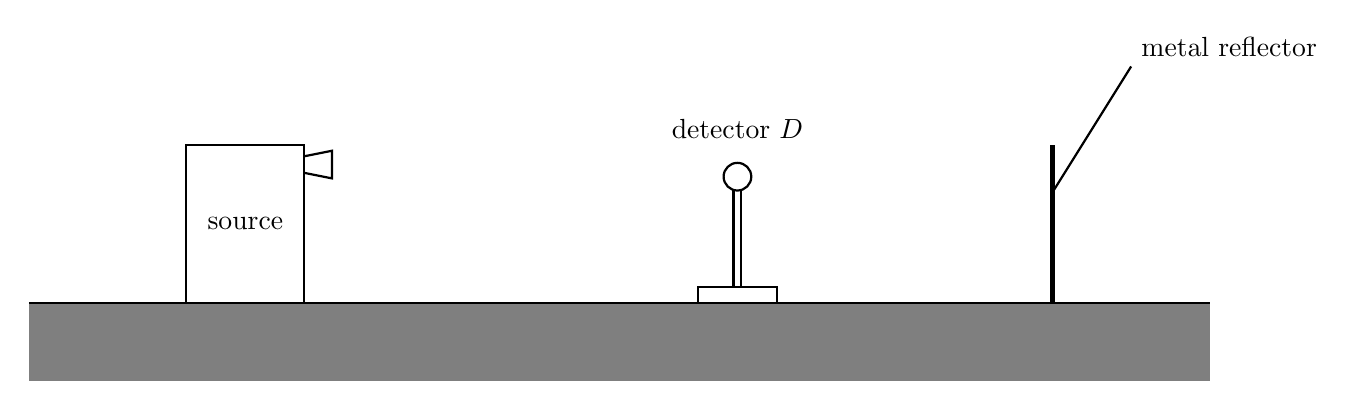
\begin{tikzpicture}[thick]
    \coordinate (source) at (2, 0);
    \coordinate (detector) at (9, 0);
    \coordinate (reflector) at (13, 0);

    \path[fill, opacity=0.5] (0, 0) rectangle (15, -1);
    \path[draw] (0, 0) -- (15, 0);

    \path[draw] (source) rectangle +(1.5, 2) node [anchor=center] (tip) {} node[midway, anchor=center] {source};
    \path[draw] ($(tip) - (0, 0.2em)$) +(0, -0.2em) -- +(1em, 0) -- +(1em, -1em) -- +(0, -0.8em);

    \begin{scope}[shift=(detector)]
      \path[draw] (-0.5, 0.2) rectangle (0.5, 0);
      \path[draw] (-0.05, 0.2) -- (-0.05, 1.6) -- (0.05, 1.6) -- (0.05, 0.2);
      \path[draw, fill=white] (0, 1.6) circle[radius=0.5em] node[above=1em] {detector $D$};
    \end{scope}

    \begin{scope}[shift=(reflector)]
      \path[draw, ultra thick] (0, 0) -- (0, 2) node[pos=0.7, anchor=center] (a) {};
      \path[draw, thick] (a.center) -- (1, 3) node[pos=1, above right] {metal reflector};
    \end{scope}
  \end{tikzpicture}

  \caption{Figure for question~\ref{q:stat-metal-reflect}}
  \label{fig:stat-metal-reflect}

  \figureruletbottom
\end{figure}

\begin{question}%
  \label{q:stat-metal-reflect}%
  \qtitle{Explain how $D$ is used to show that stationary waves are formed between reflector and wave source in figure~\ref{fig:stat-metal-reflect}}\qpoint{2}

  detector/$D$ is moved between reflector and source\hfill\point{1}\\*
  maximum, minimum/zero, (maximum… etc.) observed on meter\allowbreak/deflections\allowbreak/readings\allowbreak/measurements\allowbreak/recordings\hfill\point{1}\\*
  \NOT \refterm{node}s and \refterm{antinode}s observed.
\end{question}

\begin{question}%
  \qtitle{Describe the \term{Doppler effect}}\qpoint{1}

  \textbf{observed} \refterm{frequency} is different to source \refterm{frequency} when source moves relative to observer~\hfill\point{1}\\*
  \NOT due to change in position of source
\end{question}

\begin{question}%
  \qtitle{Describe what is meant by a \term{polarised wave}}\qpoint{2}

  vibrations are in a single direction~\hfill\point{1}\\*
  applies to transverse waves \OR normal to direction of wave energy travel / propagation~\hfill\point{1}\\*
  \NOT vibration in only one plane
\end{question}

\begin{question}%
  \qtitle{Use the principle of \refterm{superposition} to explain \textit{<some observation>}}\qpoint{2}

  the waves (that overlap) have \refterm{phase difference} of $x \si{\degree}$ / $y\ \si{rad}$ / path difference of $z \lambda$~\hfill\point{1}\\*
    constructive / destructive interference \OR displacement larger / smaller (depend on question)~\hfill\point{1}
\end{question}

\begin{question}%
  \qtitle{State what is meant by the \term{diffraction} of a wave.}\qpoint{2}

  When wave incident on/passes by/through an aperture/edge~\hfill\point{1}\\*
  it spreads (into the geometrical shadow)~\hfill\point{1}\\*
  \NOT bending\\*
  \NOT when the wave passes through an obstacle
\end{question}

\begin{question}%
  \qtitle{State what is meant by \term{interference} / \term{superposition}}\qpoint{2}

  when two (or more) waves \refterm{superpose}/meet/overlap~\hfill\point{1}\\*
  resultant displacement is the sum of the displacement of each wave~\hfill\point{1}\\*

  {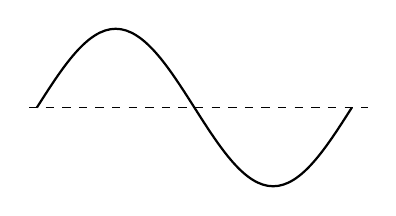
\begin{tikzpicture}[baseline=(a.center)]
    \path[thin, dashed, draw] (-0.1, 0) -- (4.2, 0);
    \path[thick, draw] (0, 0) sin (1, 1) cos (2, 0) sin (3, -1) cos (4, 0) node[pos=1, anchor=center] (a) {};
  \end{tikzpicture} \hfill $+$ \hfill 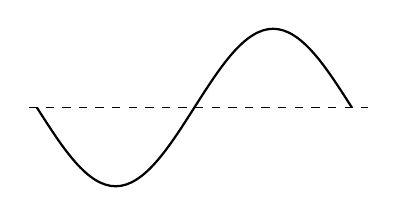
\begin{tikzpicture}[baseline=(a.center)]
    \path[thin, dashed, draw] (-0.1, 0) -- (4.2, 0);
    \path[thick, draw] (0, 0) sin (1, -1) cos (2, 0) sin (3, 1) cos (4, 0) node[pos=1, anchor=center] (a) {};
  \end{tikzpicture} \hfill $=$ \hfill 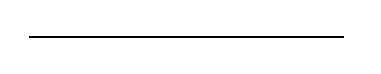
\begin{tikzpicture}[baseline=(a.center)]
    \path[thick, draw] (0, 0) -- (4, 0) node[pos=1, anchor=center] (a) {};
  \end{tikzpicture}}
\end{question}

\begin{question}%
  \qtitle{Explain the meaning of \term{coherent}}\qpoint{1}

  constant \refterm{phase difference}~\hfill\point{1}
\end{question}

\begin{question}%
  \qtitle{Explain the part played by \refterm{diffraction} in the production of the fringes in the \refterm{double slit experiment}}\qpoint{2}

  waves at (each) slit/aperture spread (into the geometric shadow)~\hfill\point{1}\\*
  (the spread) wave(s) overlap/\refterm[superposition]{superpose}/sum/meet/intersect~\hfill\point{1}
\end{question}

\begin{question}%
  \qtitle{Explain the reason why a double slit is used rather than two separate sources of light in the \refterm{double slit experiment}}\qpoint{1}

  two separate light sources are not in constant phase difference/\reftermnoindex[coherent]{coherence}\index{coherent}~\hfill\\*
  \OR waves/light from the double slit are \refterm{coherent}/have a constant phase difference~\hfill\point{1}
\end{question}

\begin{figure}[h]
  \figureruletop
  \centering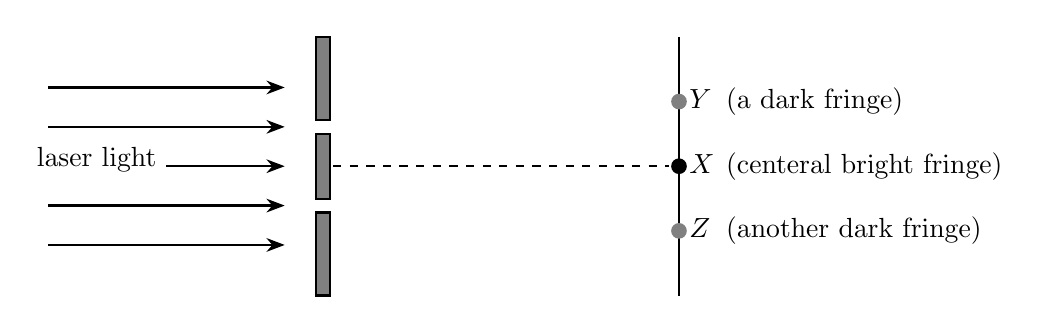
\begin{tikzpicture}[baseline=(baseline.base)]
    \def\lightarrow#1{\path [draw, -{Stealth}, thick] (0, #1) -- (3, #1)}
    \lightarrow{1};
    \lightarrow{0.5}
      node[pos=1, anchor=base west, xshift=1em] (slitline1) {};
    \lightarrow{0}
      node[midway, anchor=base east, align=right, fill=white] (baseline) {laser light}
      node[pos=1, anchor=base west, xshift=1em] (centerline) {};
    \lightarrow{-0.5}
      node[pos=1, anchor=base west, xshift=1em] (slitline2) {};
    \lightarrow{-1};

    \path [draw=black, fill=gray, thick] ([yshift=0.25em, xshift=-0.25em]slitline1) rectangle ([yshift=3.25em, xshift=0.25em]slitline1) node[pos=1, anchor=west] (top) {};
    \path [draw=black, fill=gray, thick] ([yshift=-0.25em, xshift=-0.25em]slitline1) rectangle ([yshift=0.25em, xshift=0.25em]slitline2);
    \path [draw=black, fill=gray, thick] ([yshift=-0.25em, xshift=-0.25em]slitline2) rectangle ([yshift=-3.25em, xshift=0.25em]slitline2) node[pos=1, anchor=west] (bottom) {};
    \path [draw=black, thick, dashed] ([xshift=0.5em]centerline) -- ++ (12em, 0) node[pos=1, anchor=base west] (lineright) {};

    \def\letterbox#1{\makebox[1em][l]{#1}}

    \path [draw, thick] let \p1 = (lineright), \p2 = (top), \p3 = (bottom) in (\x1, \y2) -- (\x1, \y3)

      node[midway, right, align=left] {\letterbox{$X$} (centeral bright fringe)}
      node[midway, anchor=center, shape=circle, inner sep=0.2em, fill=black, draw=none] {}

      node[pos=0.25, right, align=left] {\letterbox{$Y$} (a dark fringe)}
      node[pos=0.25, anchor=center, shape=circle, inner sep=0.2em, fill=gray, draw=none] {}

      node[pos=0.75, right, align=left] {\letterbox{$Z$} (another dark fringe)}
      node[pos=0.75, anchor=center, shape=circle, inner sep=0.2em, fill=gray, draw=none] {};
  \end{tikzpicture}

  \caption{for question~\ref{q:double-slits-q1} and~\ref{q:double-slits-q2}. Not to scale.}
  \label{fig:double-slits-x}
  \figureruletbottom
\end{figure}

\begin{question}%
  \label{q:double-slits-q1}%
  \qtitle{Explain why a bright fringe is produced at point $X$ in figure~\ref{fig:double-slits-x}.}\qpoint{2}

  waves (from slits) overlap (at point $X$)~\hfill\point{1}

  path difference (from slits to $X$) is zero\\*
  \OR phase difference (between the two waves) is zero~\hfill\point{1}\\*
  (so constructive interference gives bright fringe)

  \NOT statements that applies to all bright fringes in general -- e.g. path difference = $n \lambda$ or
  phase difference = $\SI{360}{\degree} n$.
\end{question}

\begin{question}%
  \label{q:double-slits-q2}%
  \qtitle{The intensity of the light passing through the two slits in figure~\ref{fig:double-slits-x} was initially
    the same. The intensity of the light through one of the slits is now reduced. Compare the appearance of the fringes before and after the change of intensity.}\qpoint{2}

  Any \point{2} of:\\*
  same separation/fringe width/number of fringes\\*
  bright fringes/central bright fringe/(fringe at) $X$ less bright\\*
  dark fringes/(fringe at) $Y$/$Z$ brighter

  \NOT `fringes' if it is not clear whether it refers to the dark fringes or the white fringes.
\end{question}

\begin{question}%
  \qtitle{Describe the \refterm{diffraction} of light at a \refterm{diffraction grating}}\qpoint{2}

  waves at the slits \point{1} spread (into the geometric shadow) \point{1}\\*
  \NOT light spread without the word `wave'
\end{question}

\begin{question}%
  \label{q:dffgrat-d-and-i-first}%
  \qtitle{Explain the part played by \refterm{diffraction} and \refterm[superposition]{interference} in the production of the first order maximum by the \refterm{diffraction grating}.}\qpoint{3}

  diffraction: spreading/diverging of waves/light (takes place) at (each) slit\allowbreak/element\allowbreak/gap\allowbreak/aperture~\hfill\point{1} \\*
  interference: waves (from \refterm{coherent} sources at each slit) overlap \point{1} with phase difference \SI{360}{\degree} / path difference $\lambda$ \point{1}

  See also: question~\ref{q:dffgrat-zero-and-first}
\end{question}

\begin{question}%
  \label{q:dffgrat-zero-and-first}%
  \qtitle{By reference to \refterm[superposition]{interference}, explain the zero and first order maximum in a \refterm{diffraction grating}.}\qpoint{3}

  \begin{itemize}
    \item[zero:] waves (from each slit) overlap/meet/\refterm[superposition]{superpose} \point{1} with a phase difference/path difference of zero \point{1}
    \item[first:] phase difference is \SI{360}{\degree}/path difference of $\lambda$~\hfill\point{1}
  \end{itemize}

  For the first mark, explicit mentioning that the waves \textbf{meet} or otherwise interference is necessary.

  See also: question~\ref{q:dffgrat-d-and-i-first}
\end{question}

  \defcatagory{Dynamics and Energy}

\begin{question}%
  \qtitle{Define \term{speed}}\qpoint{1}

  $\frac{\text{change in distance}}{\text{change in time}}$ \OR $\frac{\text{distance}}{\text{time}}$~\hfill\point{1}\vspace{0.5em}\\*
  \AVOID `distance over time'\\*
  \NOT `change of distance \textit{with} time'
\end{question}

\begin{question}%
  \qtitle{Define \term{velocity}}\qpoint{1}

  rate of change of \refterm{displacement} \OR $\frac{\text{change in displacement}}{\text{time (taken)}}$~\hfill\point{1}\\*
  \NOT rate of change of displacement per unit time\\*
  \AVOID `displacement over time'\\*
  \NOT `change of displacement \textit{with} time'\\*
  \NOT something with `distance'\\*
  \NOT displacement per second (just like \NOT `meter per time')

  Not to be confused with \refterm{speed}.
\end{question}

\begin{question}%
  \qtitle{Define \term{acceleration}}\qpoint{1}

  rate of change of \refterm{velocity} \OR $\frac{\text{change in \refterm{velocity}}}{\text{time (taken)}}$~\hfill\point{1}\\*
  \NOT rate of change of velocity per unit time\\*
  \NOT something with `speed'
\end{question}

\begin{question}%
  \qtitle{Define \term{force}}\qpoint{1}

  Rate of change of \refterm{momentum}~\hfill\point{1}\\*
  \NOT $F = ma$ or ``$\text{mass} \times \text{\refterm{acceleration}}$''\\*
  Definitely \NOT ``a push or pull''--this is primary grade stuff.
\end{question}

\begin{question}%
  \qtitle{Define \term{power}}\qpoint{1}

  $\frac{\text{\refterm{work} (done)}}{\text{time (taken)}}$ \OR $\frac{\text{\refterm{energy} transferred}}{\text{time (taken)}}$ \OR rate of \refterm{work} done~\hfill\point{1} \vspace{0.5em}\\*
  \NOT $\frac{\text{\refterm{energy}}}{\text{time}}$ \\*
  \AVOID `in a certain time' / `unit of time' \\*
  \AVOID `over time'
\end{question}

\begin{question}%
  \qtitle{Define \term{work} done}\qpoint{2}

  $\text{\refterm{force}} \times \text{distance moved (by force)}$~\hfill\point{1}\\*
  in the direction of the force~\hfill\point{1}
\end{question}

\begin{question}%
  \qtitle{Explain what is meant by \term{kinetic energy}.}\qpoint{1}

  energy/ability to do work a object/body/mass has due to its speed\allowbreak/velocity\allowbreak/motion\allowbreak/movement~\hfill\point{1}
\end{question}

\begin{question}%
  \qtitle{Define \term{potential energy}}\qpoint{1}

  Stored energy available to do work~\hfill\point{1}\\*
  \NOT description of any specific type of energy e.g. \refterm[gravitational potential energy]{gravitational}
\end{question}

\begin{question}%
  \qtitle{Define \term{gravitational potential energy}}\qpoint{1}

  Energy due to height/position of mass \OR distance from mass \OR
  moving mass from one point to another.~\hfill\point{1}\\*
  \NOT about `height of a body above the Earth'\\*
  \NOT about gravitational potential
\end{question}

\begin{question}%
  \qtitle{Define \term{elastic potential energy}}\qpoint{1}

  Energy (stored) due to deformation/stretching/compressing/change in shape/size~\hfill\point{1}\\*
  \NOT `the energy stored in an elastic body' without mentioning deformation\\*
  \NOT any formula
\end{question}


\begin{question}%
  \qtitle{State \term{Hooke's law}.}\qpoint{1}

  force/load is proportional to extension/compression (provided proportionality limits not exceeded)~\hfill\point{1}
\end{question}

\begin{question}%
  \qtitle{Define the \term{Young modulus}}\qpoint{1}

  $\frac{\text{\refterm{stress}}}{\text{\refterm{strain}}}$~\hfill\point{1}
\end{question}

\begin{figure}[h]%
  \figureruletop

  \centering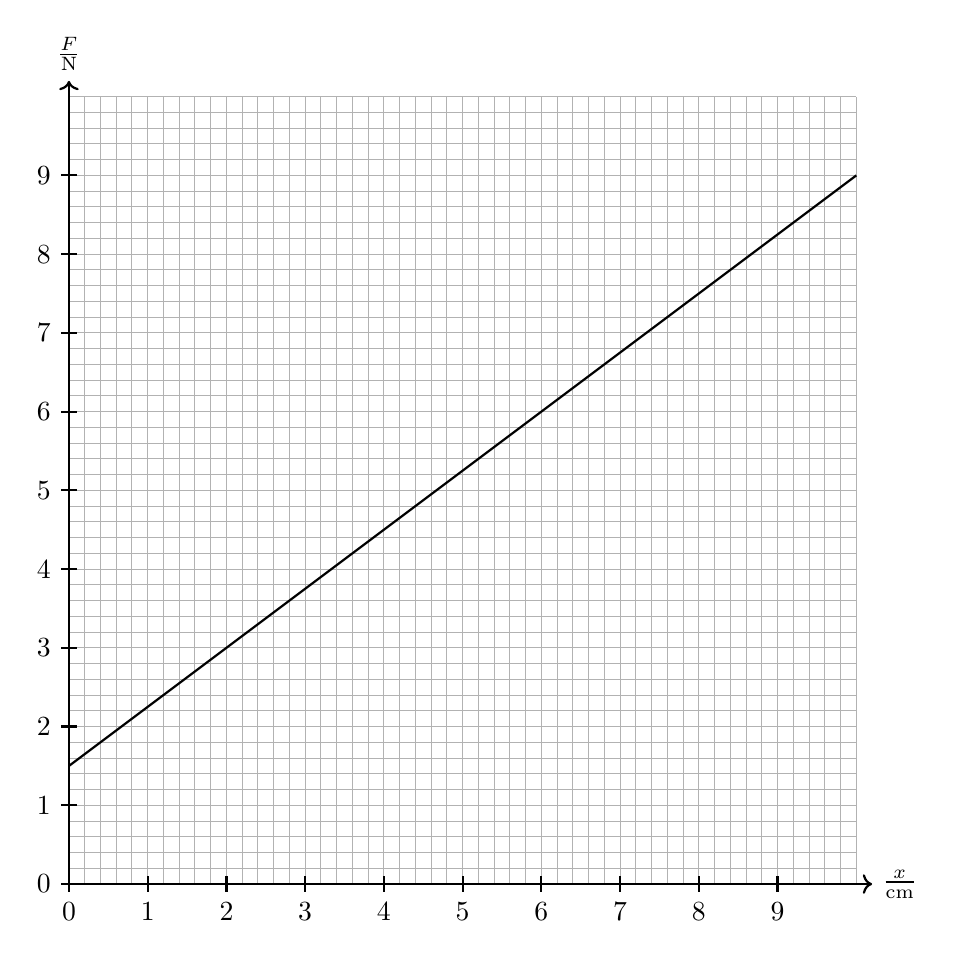
\begin{tikzpicture}
    \coordinate (topright) at (100mm, 100mm);
    \draw[help lines, color=gray!60, thin] (0, 0) grid[step=2mm] (topright);
    \path[draw, ->, thick] let \p1 = (topright) in (0, 0) -- (\x1, 0) -- ++(2mm, 0) node [pos=1, right] {$\frac{x}{\SI{}{cm}}$};
    \path[draw, ->, thick] let \p1 = (topright) in (0, 0) -- (0, \y1) -- ++(0, 2mm) node [pos=1, above] {$\frac{F}{\SI{}{N}}$};
    \foreach \y [evaluate=\y as \yN using \y/10] in {0,10,...,90} {\path[xshift=-1mm, thick, draw, x={(1mm, 0)}, y={(0, 1mm)}] (0, \y) -- ++(2, 0) node[left, pos=0] {\pgfmathprintnumber{\yN}};}
    \foreach \x [evaluate=\x as \xcm using \x/10] in {0,10,...,90} {\path[yshift=-1mm, thick, draw, x={(1mm, 0)}, y={(0, 1mm)}] (\x, 0) -- ++(0, 2) node[below, pos=0] {\pgfmathprintnumber{\xcm}};}
    \path[draw, thick] (0, 15mm) -- (100mm, 90mm);
  \end{tikzpicture}

  \caption{Figure for question~\ref{q:fx-graph}}
  \label{fig:fx-graph}

  \figureruletbottom
\end{figure}

\begin{question}%
  \label{q:fx-graph}%
  \qtitle{Use data from \textit{<some $F / x\ \text{(extension)}$ graph>} (figure~\ref{fig:fx-graph}) to show that the spring obeys \refterm{Hooke's law} for this range of extensions / compression.}\qpoint{2}

  two values of $F/x$ are calculated which are the same\\*
  \OR ratio of two forces and the ratio of the corresponding two extensions are calculated which are the same\\*
  \OR gradient of graph line calculated and coordinates of one point on the line used with straight line equation $F = mx + c$ to show $c = 0$~\hfill\point{1}

  (so) force is proportional to extension (and so \refterm{Hooke's law} obeyed)~\hfill\point{1}

  \NOT straight line $\Rightarrow$ Hooke's law obeyed, since line must cross origin.
\end{question}

\begin{question}%
  \qtitle{Describe how to determine whether the extension of the spring is \term{elastic}.}\qpoint{1}\\*
  \OR\\*
  \qtitle{State how you would check that the spring has not exceeded its \term{elastic limit}}\qpoint{1}

  remove the force/masses and if the spring returns to its original length its an elastic extension.~\hfill\point{1}\\*
  \NOT something about the extension being proportional to the force.
\end{question}

\begin{question}%
  \qtitle{For the following scenario, state and explain the changes in energy that occur.}

  \begin{itemize}
    \item [(a)] Stuff falls through liquid:\qpoint{2}

      decrease in \refterm{gravitational potential energy} due to decrease in height (since $E_p = mgh$)\\*
      increase in \refterm{thermal energy} due to \refterm{work} done against \refterm{viscous drag}\\*
      loss/change of (total) $E_p$ equal to gain/change in \refterm{thermal energy}\\*
      Any \point{2} points.
  \end{itemize}
\end{question}

\begin{question}%
  \qtitle{State the principle of \term{conservation of momentum} (linear momentum)}\qpoint{2}

  Sum/total \refterm{momentum} is constant \OR before = after~\hfill\point{1}\\*
  for an isolated system \OR with no (resultant) external force~\hfill\point{1}
\end{question}

\begin{question}%
  \qtitle{Explain what is meant by particles colliding \termnoindex[elastic collision]{elastically}\index{elastic collision}}\qpoint{1}

  the total \refterm{kinetic energy} before (the collision) is equal to the total \refterm{kinetic energy} after (the collision)~\hfill\point{1}
\end{question}

\begin{question}%
  \qtitle{Define \term{strain}}\qpoint{1}

  $\frac{\text{extension}}{\text{\textbf{original} length}}$~\hfill\point{1}
\end{question}

\begin{question}%
  \qtitle{\termnoindex[stress]{Stress}\index{stress}\ldots}

  Quantity: $\frac{\text{\refterm{force}}}{\text{\textbf{cross-sectional} area}}$~\hfill\point{1}

  Unit: \SI{}{Pa} = $\frac{\text{\refterm{force}}}{\text{area}}$~\hfill\point{1}
\end{question}

\begin{question}%
  \qtitle{State the two conditions for a system/object to be in \term{equilibrium}}\qpoint{2}

  resultant \refterm{force} (in any direction) is zero~\hfill\point{1}\\*
  resultant \refterm{torque}/\refterm{moment} (about any point) is zero \OR sum of clockwise moment and sum of anticlockwise moment is zero~\hfill\point{1}\\*
  \NOT `no turning effect'\\*
  \NOT `the forces are balanced'/`cancel'\\*
  \NOT `no forces acting'
\end{question}

\begin{question}%
  \qtitle{Define the \term{torque} of a \refterm{couple}}\qpoint{2}

  Torque is the product of one of the \refterm[force]{forces} ($F$) and the perpendicular distance ($d$) between forces.

  $\text{One of the forces} \times \text{distance}$ \point{1}\\*
  Perpendicular \point{1}

  \begin{tikzpicture}
    \coordinate (force vector) at (1, 2);
    \coordinate (origin A) at (0, 0);
    \coordinate (origin B) at ($(origin A)!1!-90:($(origin A) + (force vector)$)$);

    \path[->, draw, line width=0.1em] (origin A) -- ++(force vector) node[label=left:$F$, pos=1] {};
    \path[->, draw, line width=0.1em] (origin B) -- ++($-1*(force vector)$) node[label=right:$F$, pos=1] {};
    \path[draw=gray, dashed, thin] ($(origin A)!-2em!(origin B)$) -- ($(origin B)!-2em!(origin A)$);
    \path[draw=theme, |<->|, thick] (origin A) -- (origin B) node[midway, label={[theme]above:$d$}] {};

    \path[draw] let \p0 = (origin A) in let \p1 = ($(\p0)!0.8em!($(\p0) + (force vector)$)$), \p2 = ($(origin A)!0.8em!(origin B)$) in
      (\p1) -- ($(\p1) + (\p2) - (\p0)$) -- (\p2);
  \end{tikzpicture}
\end{question}

\begin{question}%
  \qtitle{Define the \term{moment} of a \refterm{force}}\qpoint{1}

  $\text{\refterm{force}}\ ($F$) \times \text{\textbf{perpendicular} distance}\ ($d$)\\* \text{(of line of action of force) to/from a point / pivot}$~\hfill\point{1}

  \begin{tikzpicture}
    \coordinate (force origin) at (6, 0);
    \coordinate (force vector) at (0.5, 1.5);
    \path[fill=gray, draw=black, thick] (-1mm, -1mm) rectangle ($(1mm, 1mm) + (force origin)$);
    \path[->, draw, line width=0.1em] (force origin) -- ++(force vector) node[pos=1, label=left:{$F$}] {};
    \coordinate (prep intersect) at ($($(force origin) + (force vector)$)!(0, 0)!(force origin)$);
    \path[dashed, thin, draw] ($(prep intersect)!-1em!(force origin)$) -- (force origin);
    \path[thick, draw=theme, >={Triangle[fill=theme]}, |<->|] (prep intersect) -- (0, 0) node[midway, label={[theme]below:{$d$}}] {};

    % Right angle mark
    \path[draw] let \p0 = (prep intersect) in let \p1 = ($(\p0)!0.8em!(0, 0)$), \p2 = ($(\p0)!0.8em!(force origin)$) in
      (\p1) -- ($(\p1) + (\p2) - (\p0)$) -- (\p2);
  \end{tikzpicture}
\end{question}

\begin{question}%
  \qtitle{Explain what is meant by \term{centre of gravity}}\qpoint{1}

  the point from where (all) the weight (of a body) seems to act~\hfill\point{1}\\*
  \NOT weight concentrated on this point\\*
  \NOT the point where mass acts
\end{question}

\begin{question}%
  \qtitle{Define \term{pressure}}\qpoint{1}

  $\frac{\text{\refterm{force}}}{\text{area (normal to the force)}}$~\hfill\point{1}\\*
  \NOT `cross-sectional area'
\end{question}

\begin{question}%
  \qtitle{Explain the origin of \term{upthrust} for a body in liquid}\qpoint{2}

  Pressure / force up on bottom \textbf{greater} than pressure / force down on top~\hfill\point{2}

  \point{1} for pressure on bottom \textbf{different} from pressure on top \OR pressure changes with depth.\\*
  \NOT having less density than the liquid.
\end{question}

\begin{question}%
  \qtitle{State	Newton's $n$th law of motion\ldots}

  \begin{itemize}
    \item \termnoindex[newton 1st]{$n=1$}\index{Newton's first law}: a body/mass/object continues (at rest or) at constant/uniform \refterm{velocity} unless acted on by a \textbf{resultant} \refterm{force}~\hfill\point{1}\\*
      \NOT `constant speed' without mentioning straight line motion\\*
      \NOT `uniform motion'

    \item \termnoindex[newton 2nd]{$n=2$}\index{Newton's second law}: See definition of \refterm{force}

    \item \termnoindex[newton 3rd]{$n=3$}\index{Newton's third law}: force on body A is equal in magnitude to force on body B (from A) \point{1} , in opposite directions \point{1} , of the same kind. \point{1}
  \end{itemize}
\end{question}

\def\someball{\textit{<some ball or stuff>}}%
\def\somefloor{\textit{<some floor, wall or stuff>}}%
\begin{question}%
  \qtitle{State and explain whether momentum is conserved during the collision of \someball{} with \somefloor{}}\qpoint{2}

    there is a change/gain in momentum of \somefloor{}~\hfill\point{1}\\*
    there is an equal (and opposite) change to the momentum of \someball{} so momentum is conserved~\hfill\point{1}

    \OR
    
    change of (total) momentum of \somefloor{} and \someball{} is zero\\*
    \OR (total) momentum of \someball{} and \somefloor{} before is equal to the (total) momentum after~\hfill\point{1}\\*
    so momentum is conserved~\hfill\point{1}

    \NOT not conserved for any reason such as an open system.
\end{question}

\begin{question}%
  \qtitle{Explain how the collision of two objects can support \refterm[newton 3rd]{Newton's third law}}\qpoint{2}

  change in \refterm{momentum} equal (and opposite) for the two objects~\hfill\point{1}

  \refterm{force} is change in \refterm{momentum} over time and time (of collision) is the same\\*
  hence force on the two objects are equal and opposite as for \refterm[newton 3rd]{Newton's third law}.~\hfill\point{1}
\end{question}

\begin{question}%
  \qtitle{In practice, \refterm{air resistance} is not negligible. State and explain the effect of \refterm{air resistance} on the time taken for a ball thrown upward to reach maximum height.}\qpoint{2}

  deceleration is greater/resultant force (\refterm{weight} and \refterm{friction} force) is greater~\hfill\point{1}\\*
  take less time~\hfill\point{1}
\end{question}

\begin{question}%
  \qtitle{Use the \term{kinetic model} to explain the \refterm{pressure} exerted by gases to wall of container}\qpoint{3}

  molecule collides with wall/container and there is a change in \refterm{momentum}~\hfill\point{1}\vspace{0.5em}\\*
  $\frac{\text{change in \refterm{momentum}}}{\text{time}}$ is \refterm{force} \OR $\Delta p = Ft$.~\hfill\point{1}\vspace{0.5em}\\*
  many/all/sum of molecular collisions over surface/area of container produces pressure~\hfill\point{1}
\end{question}

  \defcatagory{Particle and Nuclear Physics}

\begin{question}%
  \qtitle{Distinguish between an \term[a particle]{\ce{\alpha} particle} and a \refterm[beta+ particle]{\ce{\beta^+} particle}.}\qpoint{3}

  Any \point{3} from:

  \begin{itemize}
    \item \ce{\alpha} is 2 \refterm{proton}s and 2 \refterm{neutron}s; \ce{\beta^+} is \refterm{positron}.
    \item \ce{\alpha} has \refterm{charge} $+2e$; \ce{\beta^+} has \refterm{charge} $+e$.
    \item \ce{\alpha} has mass $4u$; \ce{\beta^+} has mass $\frac{1}{2000}u$.
    \item \ce{\alpha} made up of \refterm{hadron}s; \ce{\beta^+} made up of a \refterm{lepton}.
  \end{itemize}
\end{question}

\begin{question}%
  \qtitle{Similarity and difference between a \term[beta+ particle]{\ce{\beta^+} particle} and a \term[beta- particle]{\ce{\beta^-} particle}\ldots}

  Similarity: same (rest) mass, equal magnitude of \refterm{charge}.\\*
  Difference: opposite sign of \refterm{charge}, one is matter / electron and one is \refterm{antimatter} / antielectron / \refterm{positron}.
\end{question}

\begin{question}%
  \qtitle{State the name of the force responsible for \ce{\beta} decay.}\qpoint{1}

  \reftermnoindex[weak nuclear force]{weak (nuclear force/interaction)}\index{weak nuclear force}~\hfill\point{1} \\*
  \NOT simply `nuclear force'
\end{question}

\begin{question}%
  \qtitle{State the quantities that are conserved in a nuclear reaction.}

  Any \point{$n$} from:

  \begin{itemize}
    \item \refterm{mass-energy} \NOT separately `mass' or `energy' or `mass \textit{and} energy'
    \item \refterm{momentum}
    \item \refterm{proton number}
    \item \refterm{nucleon number}
    \item \refterm{charge}
  \end{itemize}

\end{question}

\begin{question}%
  \qtitle{State the names of the \refterm{lepton}s produced in each of the decay processes:}

  \begin{itemize}
    \item \ce{\beta^-} decay: electron and (electron) antineutrino
    \item \ce{\beta^+} decay: positron and (electron) neutrino
  \end{itemize}
\end{question}

\begin{question}%
  \qtitle{State the name of the class (group) to which each of the following belongs\ldots}

  \begin{itemize}
    \item [] \refterm{electron} / \refterm[beta- particle]{\ce{\beta} particle} / neutrino:

      \refterm{lepton}s

    \item [] \refterm{neutron} / \refterm{proton}:

      \refterm{hadron}s \OR \refterm{baryon}s
  \end{itemize}

  \textbf{Please} avoid mis-spelling.
\end{question}

\begin{question}%
  \qtitle{Explain why the sum of the kinetic energies of the carbon-13 nucleus and the \refterm[beta+ particle]{\ce{\beta^+} particle} cannot
    be equal to the total energy released by the decay process \mbox{\ce{X -> {}^{13}_{6} C + \beta^+}}.}

  a (electron) neutrino/\ce{\mathcal{V}_{(e)}} is also produced (and thus has energy)~\hfill\point{1}
\end{question}

\begin{question}%
  \qtitle{State the composition of the proton and of the neutron in terms of \refterm{quark}s.}\qpoint{1}

  \begin{itemize}
    \item proton: up up down (no strange) / $u$ $u$ $d$
    \item neutron: up down down (no strange) / $u$ $d$ $d$
  \end{itemize}
\end{question}

\begin{question}%
  \qtitle{Give one example of \ldots}

  \begin{itemize}
    \item [(i)] \refterm{hadron}: neutron \OR proton
    \item [(ii)] \refterm{lepton}: electron \OR (electron) neutrino
  \end{itemize}
\end{question}

\begin{question}%
  \qtitle{State one difference between a \term{hadron} and a \term{lepton}}\qpoint{1}

  hadrons are not fundamental particle / leptons are fundamental particle \\*
  \OR hadron made of \refterm{quark}s/lepton not made of \refterm{quark}s \\*
  \OR \reftermnoindex[strong nuclear force]{strong force/interaction}\index{strong nuclear force} acts on hadrons/does not act on leptons~\hfill\point{1}\\*
  \NOT comparing mass between \refterm{proton} and \refterm{electron}. \\*
  \NOT `only leptons experience the \reftermnoindex[weak nuclear force]{weak force}\index{weak nuclear force}'
\end{question}

\begin{question}%
  \qtitle{State what may be inferred from the following results in the \refterm[a particle scattering experiment]{\ce{\alpha} particle scattering experiment}.}

  \begin{itemize}
    \item The vast majority of \refterm[a particle]{\ce{\alpha} particle}s pass straight through the metal foil or are deviated by small angles.\qpoint{1}

    \textbf{most} of the \refterm{atom} is empty space \\*
    \OR the nucleus (volume) is (very) small \textbf{compared to the atom}~\hfill\point{1}

    \item A very small minority of \refterm[a particle]{\ce{\alpha} particle}s are scattered through angles greater than \SI{90}{\degree}.\qpoint{2}

    nucleus is (positively) charged~\hfill\point{1}\\*
    the mass/charge is concentrated / the majority of mass/charge in (very small) \refterm{nucleus} / small region/volume/core~\hfill\point{1}

  \end{itemize}

  When asked to state the results, avoid expressions such as `some', `a lot/few' or `many' particles---use `vast majority' or `vast majority'.
\end{question}

\begin{figure}[h]
  \figureruletop

  \caption{Two parallel, vertical metal plates in a vacuum are connected to a power supply, and a radioactive source emitting \refterm[a particle]{\ce{\alpha} particle}
            is placed below the plates. This is for question~\ref{q:a-experiment}~and~\ref{q:a-experiment-2}.}
  \label{fig:a-experiment}

  \centering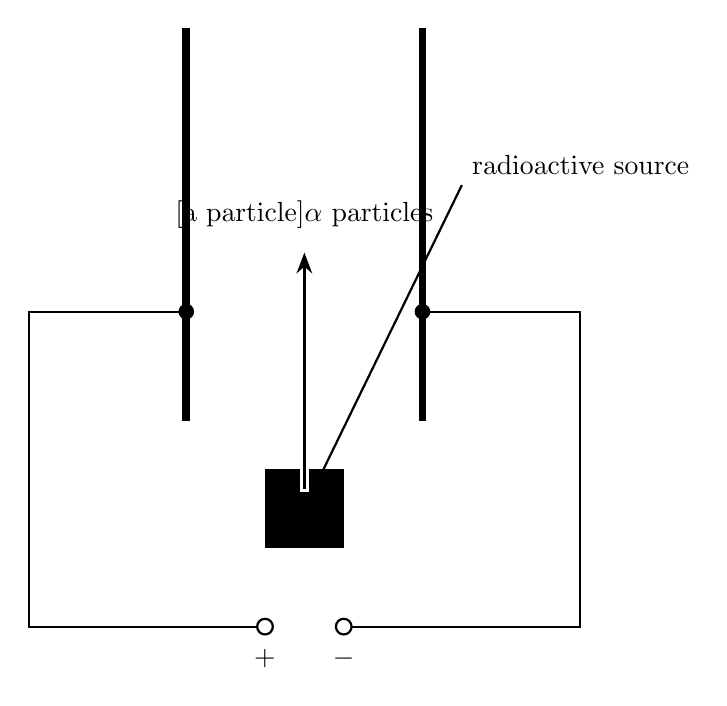
\begin{tikzpicture}
    \path[fill=black] (0.95, 0) rectangle (1.05, 5) node [below=1, midway, shape=circle, fill=black, inner sep=0.2em] (plateA) {};
    \path[fill=black] (3.95, 0) rectangle (4.05, 5) node [below=1, midway, shape=circle, fill=black, inner sep=0.2em] (plateB) {};
    \path[draw=black, thick] (plateA.center) -- ++(-2, 0) -- ++(0, -4) -- ++(3, 0) node[pos=1, anchor=center, shape=circle, draw=black, fill=white, inner sep=0.2em] (pos) {};
    \path[draw=black, thick] ($(pos.center) + (1, 0)$) -- ++(3, 0) node[pos=0, anchor=center, shape=circle, draw=black, fill=white, inner sep=0.2em] (neg) {} -- ++(0, 4) -- (plateB.center);
    \node[anchor=base] at ($(pos.center) + (0, -0.5)$) {$+$};
    \node[anchor=base] at ($(neg.center) + (0, -0.5)$) {$-$};

    \path (neg.center) -- (pos.center) node[midway, anchor=center] (supplycenter) {};
    \path[fill=black] ($(supplycenter.center) + (-0.5, 1)$) rectangle ($(supplycenter.center) + (0.5, 2)$) node[midway, anchor=center] (source) {};

    \path[draw, thick] (source.center) -- (4.5, 3) node[pos=1, anchor=south west, align=left] {radioactive source};

    \path[draw=white, line width=0.3em] ($(source.center) + (0, 0.25) + (0, -0.1em)$) -- ++(0, 3);
    \path[draw=black, -{Stealth}, line width=0.1em] ($(source.center) + (0, 0.25)$) -- ++(0, 3) node[pos=1, above=0.5em] {\refterm[a particle]{\ce{\alpha} particle}s};
  \end{tikzpicture}

  \figureruletbottom
\end{figure}

\begin{question}%
  \label{q:a-experiment}%
  \qtitle{Explain why the metal plates are placed in a \refterm{vacuum} in figure~\ref{fig:a-experiment}.}\qpoint{1}

  range of \ce{\alpha} particle is only few \SI{}{cm} in air \\*
  \OR loss of energy of the \ce{\alpha} particles due to collision with air molecules/ionisation of the air molecules~\hfill\point{1}
\end{question}

\begin{question}%
  \label{q:a-experiment-2}%
  \qtitle{The \refterm[a particle]{\ce{\alpha} particle} source in figure~\ref{fig:a-experiment} is replaced by a \refterm[beta- particle]{\ce{\beta} particle} source. By reference to the
    properties of \refterm[a particle]{\ce{\alpha} particle} and \refterm[beta- particle]{\ce{\beta} particle}, suggest three possible differences in the
    deflection observed with \refterm[beta- particle]{\ce{\beta} particle}.}\qpoint{3}

  \ce{\beta} have opposite \refterm{charge} to \ce{\alpha} therefore deflection in opposite direction~\hfill\point{1}\\*
  \ce{\beta} has a range of velocities/energies hence a number of different deflections would be seen~\hfill\point{1}\\*
  \ce{\beta} have less \refterm{mass} or $\frac{\text{\refterm{charge}}}{\text{\refterm{mass}}}$ is larger hence deflection is greater \\*
  \OR \ce{\beta} with (very) high speed (may) have less deflection~\hfill\point{1}

  There must be references to properties, such as `opposite \refterm{charge}'.
\end{question}

\begin{question}%
  \qtitle{State the \refterm{constituent particles} of the \textit{<some element>} nucleus}\qpoint{1}

  $x$ \refterm{proton}s and $y$ \refterm{neutron}s~\hfill\point{1}\\*
  \NOT $x$ electrons.
\end{question}

\begin{question}%
  \qtitle{State the \refterm{constituent particles} of \refterm[a particle]{\ce{\alpha} particle}}\qpoint{1}

  2 \refterm{proton}s and 2 \refterm{neutron}s~\hfill\point{1}\\*
  \NOT \ce{^4_2 He} / Helium / Helium nucleus
\end{question}

\begin{question}%
  \qtitle{Explain, using the law of \term{mass-energy conservation}, how \refterm{energy} is released in a \refterm{nuclear reaction}}\qpoint{2}

  (total) \refterm{mass} on left-hand side (of equation)/reactants is greater than (total) mass on right-hand side (of equation)/products~\hfill\point{1}\\*
  difference in mass is (converted to) \refterm{energy}.\hfill\point{1}
\end{question}

\begin{question}%
  \qtitle{Explain the meaning of \term{spontaneous radioactive decay}}\qpoint{1}

  (rate of decay) not affected by any external factors or changes in temperature and pressure etc.~\hfill\point{1}\\*
  \NOT decay occurred randomly / naturally
\end{question}


  \printindex
\end{document}
